\documentclass[conference]{IEEEtran}
\IEEEoverridecommandlockouts

\usepackage{cite}
\usepackage{amsmath,amssymb,amsfonts}
\usepackage{graphicx}
\usepackage{textcomp}
\usepackage{xcolor}
\usepackage{tikz}
\usepackage{url}
\usetikzlibrary{arrows.meta,positioning,calc}

\def\BibTeX{{\rm B\kern-.05em{\sc i\kern-.025em b}\kern-.08em
    T\kern-.1667em\lower.7ex\hbox{E}\kern-.125emX}}

% Helper command for image placeholders
\newcommand{\imgbox}[2]{%
  \fbox{\parbox{0.93\columnwidth}{\centering\vspace{#1}%
    {\small\sffamily\bfseries IMAGE PLACEHOLDER}\\[2pt]%
    {\scriptsize\sffamily #2}\vspace{#1}}}%
}

\begin{document}

\title{LLM-Based Knowledge Graph Construction and Retrieval for Legal Document Analysis}

\author{\IEEEauthorblockN{Samuel Bag\'{i}n, Marek Van\v{c}o}
\IEEEauthorblockA{\textit{Faculty of Electrical Engineering and Information Technology} \\
\textit{Slovak University of Technology}\\
Bratislava, Slovakia \\
xbagins@stuba.sk, marek\_vanco@stuba.sk}
}

\maketitle

\begin{abstract}
This paper presents a system for automated extraction and linking of information from legal texts into a knowledge graph with advanced semantic search. The system leverages large language models (LLMs) to transform unstructured legal documents into structured data stored in a Neo4j graph database, combined with a vector store for hybrid retrieval. A hybrid extraction approach combining open-domain detection with schema-guided extraction achieves consistent and comprehensive knowledge graphs. The GraphRAG-based search pipeline enables users to pose questions in natural language and obtain precise answers grounded in structured relationships and semantic similarity. We evaluate the processing pipeline and search accuracy on test documents, demonstrating the effectiveness of the hybrid approach.
\end{abstract}

\begin{IEEEkeywords}
knowledge graph, large language models, legal document analysis, GraphRAG, Neo4j, information extraction
\end{IEEEkeywords}

\section{Introduction}

With the growing use of Large Language Models (LLMs) across various domains, there is an increasing need for effective methods to analyze and process specific document types such as legal texts. LLMs alone often struggle with the complex structures and relationships in legal documents, leading to hallucinations and limitations in providing precise information~\cite{b1}.

We propose using LLMs to transform unstructured text into structured data stored in a knowledge graph (KG), subsequently used to answer questions via GraphRAG (Graph Retrieval-Augmented Generation)~\cite{b2}. The system combines a Neo4j~\cite{b3} graph database with a vector store for hybrid search, enabling users to ask questions in natural language and receive precise answers based on both structured relationships and semantic similarity.

The remainder of this paper is organized as follows: Section~II describes the document processing pipeline, Section~III presents the search and retrieval mechanism, Section~IV covers testing and results, and Section~V concludes the paper.

\section{Document Processing}

The processing pipeline transforms a PDF legal document into a structured knowledge graph through three main stages: preprocessing, extraction, and database insertion.

\begin{center}
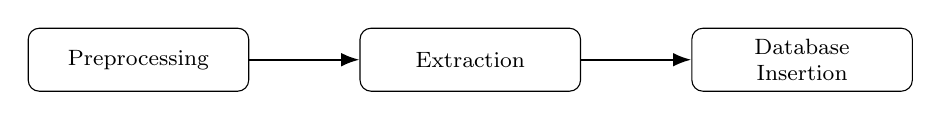
\begin{tikzpicture}[
  node distance=14mm,
  box/.style={draw, rounded corners, minimum height=8mm, minimum width=28mm, align=center, font=\footnotesize},
  arr/.style={-Latex, thick}
]
  \node[box] (pre) {Preprocessing};
  \node[box, right=of pre] (ext) {Extraction};
  \node[box, right=of ext] (db) {Database\\Insertion};
  \draw[arr] (pre) -- (ext);
  \draw[arr] (ext) -- (db);
\end{tikzpicture}
\end{center}

\subsection{Preprocessing}

The PDF document is loaded, classified, and split into chunks. Classification is performed by Google Gemini-2.5-Flash, which determines the document type (contract, law, decree, etc.) and legal domain (constitutional, financial, civil, etc.) from the first two pages. Each classification includes a confidence percentage (0--100\%).

The text is then split into chunks using \texttt{RecursiveCharacterTextSplitter} from LangChain~\cite{b4}. For open-domain extraction, chunks are 1200 tokens with 200-token overlap; for schema-guided extraction, 1024 tokens with 128-token overlap.

\subsection{Extraction}

We employ a hybrid extraction approach based on the ODKE+ study~\cite{b5}. Pure open-domain extraction yields rich but inconsistent graphs with duplicates and fragmentation (e.g., \texttt{Place} vs.\ \texttt{Location} as separate types). Pure schema-guided extraction risks missing entities not defined in the ontology. The hybrid approach combines both, achieving 98.8\% extraction accuracy~\cite{b5}.

\begin{center}
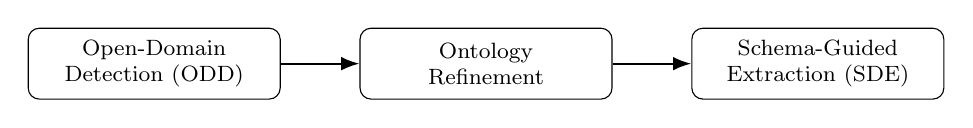
\begin{tikzpicture}[
  node distance=10mm,
  box/.style={draw, rounded corners, minimum height=9mm, minimum width=32mm, align=center, font=\footnotesize},
  arr/.style={-Latex, thick}
]
  \node[box] (det) {Open-Domain\\Detection (ODD)};
  \node[box, right=of det] (onto) {Ontology\\Refinement};
  \node[box, right=of onto] (extr) {Schema-Guided\\Extraction (SDE)};
  \draw[arr] (det) -- (onto);
  \draw[arr] (onto) -- (extr);
\end{tikzpicture}
\end{center}

\subsubsection{Open-Domain Detection (ODD)}
Each chunk is processed in parallel by an asynchronous agent using GPT-4o~\cite{b6}, which extracts every possible entity and relationship. This reveals entities not predefined in any ontology that may be crucial. The ontology dynamically adapts based on the classified document type and legal domain. The output is a schema of node and relationship type lists.

\subsubsection{Ontology Refinement}
The extracted schema is compared against a predefined reference ontology (consistent across Slovak law, e.g., \texttt{Person}, \texttt{Law}, \texttt{Paragraph}) or the existing graph schema. This ensures consistency, prevents semantically similar but differently named types (e.g., \texttt{REGULATES} vs.\ \texttt{REGULATED}), and eliminates duplicates. Gemini-2.5-Flash is used for this reasoning task.

\subsubsection{Schema-Guided Extraction (SDE)}
The most precise step: each chunk is processed in parallel with the refined ontology provided to the LLM. The agent extracts consistent entities and relationships, returning \texttt{GraphDocument} objects. The result is a rich, consistent knowledge graph where chunks link to documents via \texttt{IN\_DOCUMENT} and to entities via \texttt{HAS\_ENTITY} relationships.

\begin{figure}[!t]
\centering
\imgbox{8mm}{Neo4j graph visualization showing Document, Chunk, and Entity nodes connected by IN\_DOCUMENT, HAS\_CHUNK, and domain-specific relationships (e.g., CONTAINS, REGULATES)}
\caption{Knowledge graph structure: document, chunk, and entity relationships.}
\label{fig:graph_structure}
\end{figure}

\subsection{Database Insertion}

Data are inserted into two databases. The \textbf{graph database} (Neo4j) stores \texttt{GraphDocument} objects where each entity has a unique \texttt{elementId}, labels, and properties; relationships contain type, source, and target identifiers. The \textbf{vector database} (Neo4jVector) stores entity and relationship embeddings generated by OpenAI's \texttt{text-embedding-3-large} model. These embeddings enable semantic search via cosine similarity and are linked to the graph database through shared \texttt{elementId} values.

\begin{figure}[!t]
\centering
\imgbox{8mm}{Side-by-side: left -- Neo4j graph with entity nodes and relationships; right -- vector store entries with embeddings linked via elementId}
\caption{Dual database architecture: graph DB and vector store linked via \texttt{elementId}.}
\label{fig:dual_db}
\end{figure}

\section{Search and Retrieval}

To answer user questions, the system employs a hybrid GraphRAG approach combining knowledge graph traversal with semantic vector search. The pipeline executes the following steps:

\begin{center}
\resizebox{\columnwidth}{!}{
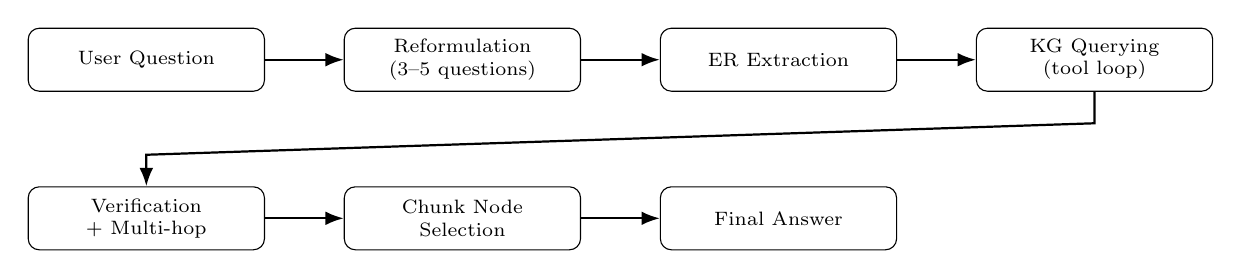
\begin{tikzpicture}[
  node distance=8mm and 10mm,
  box/.style={draw, rounded corners, align=center, minimum width=30mm, minimum height=8mm, inner sep=3pt, font=\scriptsize},
  arr/.style={-Latex, thick}
]
  \node[box] (uq) {User Question};
  \node[box, right=of uq] (rq) {Reformulation\\(3--5 questions)};
  \node[box, right=of rq] (svo) {ER Extraction};
  \node[box, right=of svo] (kg) {KG Querying\\(tool loop)};

  \node[box, below=12mm of uq] (mh) {Verification\\+ Multi-hop};
  \node[box, right=of mh] (ch) {Chunk Node\\Selection};
  \node[box, right=of ch] (ans) {Final Answer};

  \draw[arr] (uq) -- (rq);
  \draw[arr] (rq) -- (svo);
  \draw[arr] (svo) -- (kg);
  \draw[arr] (kg.south) -- ++(0,-4mm) -- ($(mh.north)+(0,4mm)$) -- (mh.north);
  \draw[arr] (mh) -- (ch);
  \draw[arr] (ch) -- (ans);
\end{tikzpicture}
}
\end{center}

\textbf{Question Reformulation.} The LLM generates 3--5 reformulations of the original question, each phrasing the key information differently to maximize retrieval coverage from the graph database.

\textbf{Entity-Relationship Extraction.} For each reformulated question, the LLM extracts all possible entities and relationships using open-domain extraction, regardless of type.

\textbf{Knowledge Graph Querying.} For each extracted entity and relationship, semantically similar counterparts are found in the vector database via \texttt{elementId} linkage. The LLM generates Cypher queries iteratively, executing them through a tool with restricted database access.

\textbf{Verification and Multi-hop Reasoning.} The LLM analyzes query results for relevance and completeness. If information is fragmented, multi-hop reasoning activates: traversing indirect entity relations (e.g., person $\rightarrow$ contract $\rightarrow$ law), supplementing context via further iterations, and eliminating hallucinations by verifying facts against the graph structure.

\textbf{Chunk Node Selection.} For all discovered nodes, associated \texttt{Chunk} nodes are retrieved via \texttt{HAS\_CHUNK} relationships, providing source text context.

\textbf{Final Answer Generation.} The answer is synthesized from the original question, reformulations, graph results, chunk texts, and the system prompt, processed by Gemini-2.5-Flash with its large context window.

\begin{figure}[!t]
\centering
\imgbox{8mm}{Complete search example: user question, generated Cypher query, returned graph nodes/relationships, and final synthesized answer}
\caption{End-to-end search pipeline example.}
\label{fig:search_example}
\end{figure}


\section{Testing and Results}

The system was tested on \textit{Romeo and Juliet} as a controlled case for both processing and search evaluation.

\subsection{Processing Evaluation}

Initial open-domain extraction yielded a rich but inconsistent graph. Schema-guided extraction using a refined schema from the open-domain results produced a consistent graph with approximately the same entity count:
\begin{equation}
N_{\text{ODD}} = 2536 \approx N_{\text{SDE}} = 2512
\end{equation}

Converting from synchronous to asynchronous processing reduced time approximately 6$\times$:
\begin{equation}
T_{\text{sync}} = 12\,\text{min},\quad T_{\text{async}} = 2\,\text{min}
\end{equation}

\begin{figure}[!t]
\centering
\imgbox{8mm}{Bar chart comparing ODD vs SDE: entity count (2536 vs 2512), processing time sync vs async (12\,min vs 2\,min), number of inconsistent relationship types}
\caption{ODD vs.\ SDE: entity count and processing time comparison.}
\label{fig:processing_comparison}
\end{figure}

\subsection{Search Evaluation}

An iterative querying agent with restricted graph database access was used to verify data quality. Query processing time ranged from 20~seconds to 4~minutes. The agent consistently found relevant data and produced accurate answers.

For the question \textit{``Which characters belonging to the Capulet house are in love with a character from the Montague house?''}, the system correctly identified \texttt{Juliet}. However, open-domain extraction revealed relationship inconsistency: instead of a single \texttt{LOVES} relationship, five variants existed (\texttt{LOVES}, \texttt{IN\_LOVE\_WITH}, \texttt{EXPRESSES\_FEELING\_FOR}, \texttt{LOVER}, \texttt{LOVE}), demonstrating the importance of ontology refinement.

\begin{figure}[!t]
\centering
\imgbox{8mm}{Neo4j subgraph: Juliet and Romeo nodes connected by LOVES, linked to Capulet and Montague house nodes via BELONGS\_TO}
\caption{Query result: cross-house relationships between Juliet and Romeo.}
\label{fig:romeo_query}
\end{figure}

Testing on this controlled dataset helped refine the system before deployment on Slovak legal documents from Slov-Lex~\cite{b7}.

\section{Conclusion}

This work presented a system for automated knowledge graph construction from legal documents using a hybrid LLM-based extraction pipeline. The combination of open-domain detection with schema-guided extraction produces rich and consistent knowledge graphs. The GraphRAG-based search pipeline leverages both graph traversal and semantic similarity for accurate question answering.

Testing demonstrated that the hybrid approach maintains entity richness while improving consistency, and asynchronous processing reduces computation time by 6$\times$. Future work includes prompt optimization, a web-based user interface, and extending coverage to the full breadth of Slovak legal documentation.


\section*{Acknowledgment}

This paper was supported by DISIC (09I05-03-V2), NEXT (ERASMUS-EDU-2023-CBHE-STRAND-2), EULiST (ERASMUS), CYB-FUT (ERASMUS+), InteRViR (VEGA 1/0605/23).

\begin{thebibliography}{00}
\bibitem{b1} Y. Yao, J. Duan, K. Xu, Y. Cai, Z. Sun, and Y. Zhang, ``A survey on large language model (LLM) security and privacy: The good, the bad, and the ugly,'' \textit{High-Confidence Computing}, vol.~4, no.~2, 2024, Art. no. 100211.
\bibitem{b2} D. Edge \textit{et al.}, ``From local to global: A graph RAG approach to query-focused summarization,'' arXiv preprint arXiv:2404.16130, 2024.
\bibitem{b3} Neo4j, Inc., ``Neo4j graph database,'' [Online]. Available: https://neo4j.com/
\bibitem{b4} LangChain, Inc., ``LangChain documentation,'' [Online]. Available: https://docs.langchain.com/
\bibitem{b5} Q. Xia, H. Ye, and M.~Sap, ``ODKE+: Ontology-guided open-domain knowledge extraction with LLMs,'' arXiv preprint arXiv:2509.04696, 2025.
\bibitem{b6} OpenAI, ``GPT-4o model card,'' 2024. [Online]. Available: https://openai.com/
\bibitem{b7} Slov-Lex, ``Legal and information portal,'' Ministry of Justice of the Slovak Republic. [Online]. Available: https://www.slov-lex.sk/
\end{thebibliography}

\end{document}
